\clearpage
\setcounter{page}{1}

\begin{table*}[h]
  \centering
  \sisetup{table-format=1.0} % adjust to your needs
  \begin{tabularx}{\textwidth}{
      c     % Method
      c                 % Certifiable
      c                 % Fast cal.
      c                 % Fast test
      c                 % l1, linf norm
      c                 % Poisoning
      S[table-format=1.0] % Nb hyperparams
    }
    \toprule
    Method & Certifiable & Fast cal. & Fast test & \(\ell_1,\,\ell_\infty\) & Poisoning & {Nb hyperparams} \\
    \midrule
    \emph{aPRCP}~\cite{prcp}               & \impossible & \impossible & \possible   & \impossible & \impossible & 2 \\
    \emph{RSCP}~\cite{rscp}               & \impossible & \impossible & \impossible & \possible   & \impossible & 3 \\
    \emph{RSCP}+ (PTT/RCT)~\cite{rscp_plus}
                                   & \possible   & \impossible & \impossible & \possible   & \impossible & 4 (6) \\
    \emph{CAS}~\cite{cas}                 & \possible   & \impossible & \impossible & \possible   & \possible   & 2 \\
    \emph{VRCP-I}~\cite{vrcp}             & \possible   & \possible   & \impossible & \possible   & \impossible & 2 \\
    \emph{VRCP-C}~\cite{vrcp}             & \possible   & \impossible & \possible   & \possible   & \impossible & 2 \\
    \emph{lip-rcp}                           & \possible   & \possible   & \possible   & \impossible & \possible   & 2 \\
    \bottomrule
  \end{tabularx}
  \caption{Comparison of certified robustness methods. Note that aPRCP is not certifiable without assumptions on the adversarial distribution. See Section~\ref{par:hyperparams} for details on hyperparameter counts.}
  \label{tab:huge_table}
\end{table*}


\section{On the Lower Bound of \citet[Theorem~2]{rscp}}
\label{app:GendlerMistake}

Unfortunately, it seems that a subtle mathematical mistake was left aside in Theorem~2 by \citet{rscp}. It can be seen in the statement and in the proof.

In the statement, the deterministic quantity $\mathbb{P}\bigl[Y_{n+1} \in \mathcal{C}(\Tilde{X}_{n+1})\bigr]$ is bounded from below by the random quantity $\tau$ (note that $\tau$ depends on the calibration data); this lower bound can thus fail in general.\footnote{This could make sense if the probability $\mathbb{P}\bigl[Y_{n+1} \in \mathcal{C}(\Tilde{X}_{n+1})\bigr]$ were conditional on the calibration data, but it is not the case in the proof: the probability is with respect to the joint distribution of $(X_i,Y_i)_{1 \leq i \leq n+1}$.}

In the proof, which appears in \citet[Appendix S1, Proof of theorem~2]{rscp}, the authors use Lemma~2 by \citet{romano2019conformalized} which only holds for deterministic values of $\tau$ (or $\alpha$, following the notation in \citealt{romano2019conformalized}). Since $\tau$ is random, their lemma can unfortunately not be used here.

\section{Proof of Theorem~\ref{thm:robustcoverageuniform}}
\label{app:new-proof}
Let $\mathcal{X}\subset\R^d$ (Borel subset) and $\norm{\cdot}$ a norm on $\R^d$. Let also $\mathcal{Y}=\{1,\cdots,K\}$ and $s:\mathcal{X}\times\mathcal{Y}\rightarrow\R$ be a measurable function (non-conformity score).

For any $x\in\mathcal{X}$ and $\epsilon \geq 0$, we set $\bouleps(x):=\left\{ \tilde{x} \in \mathcal{X} : \norm{\tilde{x} - x} \leq \epsilon\right\}$.

There are some minor measurability subtleties in the paper and the following proof, which are overlooked here for readability, but discussed in Section~\ref{sec:measurability}.

\subsection{On the continuity of $\covmax$ and $\covmin$}
\label{subsec:continuity}

\paragraph{In this section and the next}
We assume that $\CalDataset$ is fixed, so that $s(\cdot, \cdot)$ and $q_\alpha$ are deterministic. All probabilities or expectations below are taken w.r.t. the random draws of $\HoldoutDataset$ and/or $(\XYt)$. \footnote{In fact, we also work conditionally to the training set, which is treated as deterministic in all the paper.} Furthermore, since in our paper $(\CalDataset)$ is independent from $(\HoldoutDataset,(\XYt))$, all inequalities below translate into inequalities that are valid for a.e. $\CalDataset$, provided that $\mathbb{P}(\cdot)$ and $\Ex{\cdots}$ are replaced with $\mathbb{P}(\cdots | \CalDataset)$ and $\Ex{\cdots | \CalDataset}$.\\

We now study $\covmax$ and $\covmin$. For $\epsilon\geq 0$, recall that 
$$
\covmax(\epsilon) = \mathbb{P}\left(\sie(\XYt)\leq q_\alpha\right)\quad \textrm{and} \quad \covmin(\epsilon)=\mathbb{P}\left(\sse(\XYt)\leq q_\alpha\right) \;,
$$
where, in order to emphasize the dependency in $\epsilon$, we wrote
\[
\sie(x,y)=\inf\limits_{\tilde{x}\in\bouleps(x)} s(\tilde{x},y) \quad \textrm{and} \quad  \sse(x,y) = \sup\limits_{\tilde{x}\in\bouleps(x)} s(\tilde{x},y) \;.
\]

\begin{proposition}
\label{prop:continuityGamma}
    Assume that A1 and A2 from \ref{assum:X-s} hold true. Then, $\covmax$ is right-continuous on $[0,+\infty)$ and $\covmin$ is left-continuous on $(0,+\infty)$.
\end{proposition}
\begin{proof}
    We start with $\covmax$. Let $\epsilon\geq 0$ and $\eta>0$. We show that there exists $\delta>0$ s.t. $\covmax(\epsilon+\delta)\leq\covmax(\epsilon)+\eta$, which will (by monotonicity of $\covmax$) imply that $\abs{\covmax(\epsilon^\prime)-\covmax(\epsilon)}\leq \eta$ for all $\epsilon^\prime\in[\epsilon, \epsilon+\delta]$.

    Let $K\subset \mathcal{X}$ be any compact set such that $\mathbb{P}(\Xt \in K) \geq 1 - \frac{\eta}{2}$.

    By right-continuity of the cdf $t\mapsto F_\epsilon(t):=\mathbb{P}\left(\sie(\XYt)\leq t | \Xt \in K \right)$, there exists $\rho>0$ s.t. $F_\epsilon (q_\alpha + \rho) \leq F_\epsilon(q_\alpha) + \frac{\eta}{2}$.

    We now use the fact that, for each $y\in\mathcal{Y}$ (with $\mathcal{Y}$ finite), the function $s(\cdot, y)$ is continuous and thus uniformly continuous on the compact set $K_{\epsilon+1}:=\left\{ x+u : x\in K, u\in\R^d, \norm{u}\leq\epsilon+1\right\}$. Therefore, there exists $\delta\in(0,1)$ s.t., 
    \begin{equation}
        \label{eq:conti}
        \forall y \in \mathcal{Y}, \forall x, x^\prime \in K_{\epsilon+1}, \norm{x-x^\prime}\leq \delta \implies \abs{s(x,y)-s(x^\prime, y)}\leq\rho.
    \end{equation}
    Note that, for any $y\in\mathcal{Y}$ and $x\in K$, by \eqref{eq:conti} above,
    \begin{equation}
    \label{eq:sie-ineq}
        \sie(x,y)=\inf\limits_{\tilde{x}\in\bouleps(x)}s(\tilde{x},y)\leq\inf\limits_{\tilde{x}\in\boule_{\epsilon+\delta}(x)}s(\tilde{x},y)+\rho = \underline{s}_{\epsilon+\delta}(x,y)+\rho.
    \end{equation}
    \begin{figure}
        \centering
        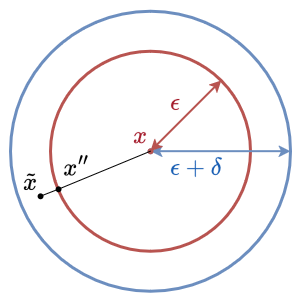
\includegraphics[width=0.3\columnwidth]{proof_illustration.png}
        \caption{Illustration of the proof of \eqref{eq:sie-ineq}. On the ball $\mathcal{B}_{\epsilon + \delta} (x)$, the score $x \mapsto s(x,y)$ is minimized at some $\Tilde{x}$. On the smaller ball $\mathcal{B}_{\epsilon}(x)$, the minimum can only be larger, but not larger than $s(x'',y)$ which is close to $s(\Tilde{x},y)$ by continuity of $s(\cdot,y)$.}
        \label{fig:preuve-2}
    \end{figure}
    This follows from Figure \ref{fig:preuve-2}. More formally, let $\tilde{x}\in\boule_{\epsilon+\delta}(x)$ be such that $s(\tilde{x},y)=\underline{s}_{\epsilon+\delta}(x,y)$. Inequality \eqref{eq:sie-ineq} is immediate if $\norm{\tilde{x}-x} \leq \epsilon$. We thus assume without loss of generality that $\norm{\tilde{x}-x}>\epsilon$. Then, let $x^{\prime\prime}\in[x,\tilde{x}] \subset\mathcal{X} $ be such that $\norm{x^{\prime\prime}-x}=\epsilon$ (recall that $\mathcal{X}$ is convex). In this case $\norm{\tilde{x}-x^{\prime\prime}}\leq\delta$ and thus (by \eqref{eq:conti}) $s(x^{\prime\prime},y)\leq s(\tilde{x}, y)+\rho$ which implies $\underline{s}_\epsilon (x,y)\leq s(x^{\prime\prime},y) \leq \underline{s}_{\epsilon+\delta}(x,y)+\rho$. This concludes the proof of \eqref{eq:sie-ineq}.

    We are ready to conclude:
    \begin{equation*}
        \begin{aligned}
        & \covmax(\epsilon+\delta)=\mathbb{P}\left(\underline{s}_{\epsilon+\delta}\left(\Xt, \Yt\right) \leq q_\alpha\right) \\
        & \leq \mathbb{P}\left(\Xt \in K\right) \cdot \mathbb{P}\left(\underline{s}_{\epsilon+\delta}\left(\Xt, \Yt\right) \leq q_\alpha \mid \Xt \in K\right)+\mathbb{P}\left(\Xt \notin K\right) \\
        & \stackrel{\text{by }\eqref{eq:sie-ineq}}{\leq} \mathbb{P}\left(\Xt \in K\right) \cdot \underbrace{\mathbb{P}\left(\underline{s}_{\epsilon}\left(\Xt, \Yt\right) \leq q_\alpha+\rho \mid \Xt \in K\right)}_{=F_{\epsilon}\left(q_\alpha+\rho\right) 
        \leq F_{\epsilon}\left(q_\alpha\right)+\frac{\eta}{2}}+\frac{\eta}{2}\\
        & \leq \mathbb{P}\left(\Xt \in K\right) \cdot\left[\mathbb{P}\left(\left.\sie\left(\Xt,\Yt\right) \leq q_\alpha \right\rvert\, \Xt \in K\right)+\frac{\eta}{2}\right]+\frac{\eta}{2} \\
        & \leq \mathbb{P}\left(\sie\left(\Xt, \Yt\right) \leq q_\alpha\right)+\eta \\
        & =\covmax(\epsilon)+\eta
        \end{aligned}
    \end{equation*}

    This entails $\abs{\covmax(\epsilon^\prime)-\covmax(\epsilon)}\leq\eta$ for all $\epsilon^\prime \in [\epsilon,\epsilon+\delta]$, and proves that $\covmax$ is right-continuous.

    The proof that $\covmin$ is left-continuous follows from similar arguments. Put briefly: for all $\epsilon>0$ and $\eta>0$, there exist a compact subset $K\subset\mathcal{X}$ and two real numbers $\rho>0$ and $\delta\in(0,\epsilon)$ such that
    \begin{equation*}
        \begin{aligned}
            & \covmin(\epsilon-\delta)=\mathbb{P}\left(\bar{s}_{\epsilon-\delta}\left(\Xt, \Yt\right) \leq q_\alpha\right) \\
        & \leq \mathbb{P}\left(\Xt \in K\right) \cdot \mathbb{P}\left(\bar{s}_{\epsilon-\delta}\left(\Xt, \Yt\right) \leq q_\alpha \mid \Xt \in K\right)+\mathbb{P}\left(\Xt \notin K\right) \\
        & \stackrel{s(\cdot,y) \text{ u.c. on } K}{\leq} \mathbb{P}\left(\Xt \in K\right) \cdot \mathbb{P}\left(\bar{s}_{\epsilon}\left(\Xt, \Yt\right) \leq q_\alpha+\rho \mid \Xt \in K\right)+\frac{\eta}{2}\\
        & \leq \mathbb{P}\left(\Xt \in K\right) \cdot\left[\mathbb{P}\left(\left.\sse\left(\Xt,\Yt\right) \leq q_\alpha \right\rvert\, \Xt \in K\right)+\frac{\eta}{2}\right]+\frac{\eta}{2} \\
        & \leq \mathbb{P}\left(\sse\left(\Xt, \Yt\right) \leq q_\alpha\right)+\eta \\
        & =\covmin(\epsilon)+\eta
        \end{aligned}
    \end{equation*}
    
    \end{proof}

    \paragraph{N.B.}
    The proof is a little easier if $s(\cdot,y)$ is uniformly continuous on $\mathcal{X}$ (e.g. if $\mathcal{X}$ is compact or $s(\cdot,y)$ is Lipschitz). In that case, there is no need to work conditionally on $\left\{\Xt \in K \right\}$.

    \subsection{Concentration of $\covmaxm$ around $\covmax$}

    Let $\HoldoutDataset=\left( X_i, Y_i \right)_{1\leq i\leq m}$ be $m\geq 2$ independent copies of $(\XYt)$.

    For $\epsilon>0$, let 
    $$
        \covmaxm(\epsilon) := \frac{1}{n} \sum\limits_{i=1}^{m}\mathds{1}_{\sie(\XYi)\leq q_\alpha}.
    $$

    Let $\delta\in(0,1)$. Since $m\covmaxm(\epsilon)\sim \mathrm{Binomial}(m,\covmax(\epsilon))$, the estimator
    $$
        \covmaxmp(\epsilon, \delta) := \max \left\{ p\in[0,1] : \mathrm{Bin}_{m,p}(m\covmaxm(\epsilon))\geq \delta\right\},
    $$
    where $\mathrm{Bin}_{m,p}$ is the c.d.f. of $\mathrm{Binomial}(m,p)$. This estimator satisfies (e.g., Theorem~3.3 by \citealt{langford2005tutorial}), for all $\epsilon \geq 0$ and $\delta\in(0,1)$,
    \begin{equation}
        \label{eq:ucb}
        \mathbb{P}\left(\covmax(\epsilon)\leq\covmaxmp(\epsilon,\delta)\right)\geq 1-\delta
    \end{equation}

    Applying \eqref{eq:ucb} $m-1$ times with properly chosen values of $\epsilon$ (of a quantile flavor), and using the fact that both $\covmax$ and $\covmaxmp(\cdot, \delta)$ are a.s. right-continuous and non-decreasing, we obtain the following ``uniform'' concentration inequality.

    \begin{theorem}
    \label{thm:appendix-thm-1}
        Assume that A1 and A2 from \ref{assum:X-s} hold true.
        Let $(\XYi)_{1\leq i \leq m}$ be $m\geq 2$ independent copies of $(\XYt)$. Then:
        $$
            \mathbb{P}\left(\forall \epsilon\geq0, \covmax(\epsilon)\leq\covmaxmp(\epsilon,\frac{\delta}{m-1})+\frac{1}{m}\right)\geq 1-\delta.
        $$
    \end{theorem}
    As seen in the proof below, $\covmax$ and $\covmaxmp(\cdot, \delta)$ are right-continuous a.s., so that the above probability is well defined (the $\forall\epsilon$ can be replaced with a countable $\forall\epsilon_k$).
    \begin{proof}
        We proceed in three steps.
        \paragraph{Step 1: right-continuity of $\covmax$ and $\covmaxmp(\cdot, \delta)$}
        \begin{itemize}
            \item the fact that $\covmax$ is right-continuous follows from Subsection \ref{subsec:continuity}.
            \item likewise, using this result with the empirical distribution $\frac{1}{m}\sum_{i=1}^{m}\delta_{(\XYi)}$, we can see that the random function $\epsilon\mapsto\covmaxm(\epsilon)$ is right-continuous, and thus locally constant to the right of any $\epsilon\geq0$. This implies that $\epsilon\mapsto\covmaxmp(\epsilon,\delta)$ is also right-continuous on $[0,+\infty)$.
        \end{itemize}

        \paragraph{Step 2: pointwise concentration and union bound}
        For every $k\in\{1,\cdots,m-1\}$, we set $\epsilon_k := \inf \left\{ \epsilon \geq 0 : \covmax(\epsilon)\geq\frac{k}{m}\right\}$, with the convention that $\inf \varnothing = +\infty$. Let also $\epsilon_m := +\infty$.
        Note that $0\leq\epsilon_1\leq \epsilon_2 \leq \cdots\leq \epsilon_m\leq +\infty$ and that $\covmax(\epsilon_k)\geq\frac{k}{m}$ whenever $\epsilon_k < \infty$ (by right-continuity of $\covmax$ on $[0,+\infty)$).
        
        First note that, if $\epsilon_1=+\infty$, then $\covmax(\epsilon)<\frac{1}{m}$ for all $\epsilon \geq 0$ by def of $\epsilon_1$). 
        In this case, the conclusion of Theorem \ref{thm:appendix-thm-1} would hold trivially.

        We can thus assume without loss of generality that $\epsilon_1<+\infty$, and set 
        $$
            K:=\max\left\{k\in\{1,\cdots,m-1\}: \epsilon_k <+\infty\right\}.
        $$
        Note that $0\leq\epsilon_1\leq\cdots\leq\epsilon_K<\epsilon_{K+1}=\cdots=\epsilon_m=+\infty$.

        Combining \eqref{eq:ucb} with a union bound, and using $K\leq m-1$, we get:

        \begin{equation}
            \label{eq:union-bound}
            \mathbb{P}\left(\forall k\in\{1,\cdots,K\}, \covmax(\epsilon_k)\leq\covmaxmp(\epsilon_k, \frac{\delta}{m-1})\right)\geq 1-\frac{K\delta}{m-1}\geq 1-\delta.
        \end{equation}

        \paragraph{Step 3: bridging the gaps}
        
        Let $\Omega_\delta := \left\{ \forall k \in \{1,\cdots,K\}, \covmax(\epsilon_k)\leq\covmaxmp(\epsilon_k, \frac{\delta}{m-1} \right\}$ be the event appearing in \eqref{eq:union-bound}. 
        We now work on the event $\Omega_\delta$.

        Let $\epsilon\geq\epsilon_1$. Note that $\epsilon$ belongs to one of the following K disjoint (possibly empty) intervals:
        $$
            I_k = [\epsilon_k, \epsilon_{k+1}), k\in\{1,\cdots,K\} \quad \text{(by convention, $I_k=\varnothing$ if $\epsilon_k=\epsilon_{k+1}$)}.
        $$
        We let $k\in\{1,\cdots,K\}$ be such that $\epsilon\in I_k$, i.e., $\epsilon_k \leq \epsilon < \epsilon_{k+1}$.

        Recall that $\covmax(\epsilon_k)\geq\frac{k}{m}$, and note that $\covmax(\epsilon)\leq\frac{k+1}{m}$. 

        Therefore,
        \begin{equation*}
            \begin{aligned}
                \covmax(\epsilon) &\leq \frac{k+1}{m}\\
                &\leq \covmax(\epsilon_k) + \frac{1}{m}\\
                &\leq \covmaxmp(\epsilon_k,\frac{\delta}{m-1})+\frac{1}{m} & \text{(we work on $\Omega_\delta$)}\\
                &\leq \covmaxmp(\epsilon, \frac{\delta}{m-1})+\frac{1}{m} &\text{(by $\epsilon_k \leq \epsilon$ and monotonicity of $\covmaxmp(\cdot,\frac{\delta}{m-1}))$}
            \end{aligned}
        \end{equation*}

        Since we also have $\covmax(\epsilon)\leq\frac{1}{m}$ if $\epsilon_1>0$ and $\epsilon \in [0,\epsilon_1)$ (by definition of $\epsilon_1$), we just proved that, on the event $\Omega_\delta$,
        $$
            \forall \epsilon \geq 0, \covmax(\epsilon) \leq \covmaxmp(\epsilon, \frac{\delta}{m-1})+\frac{1}{m}.
        $$
        Recalling that $\mathbb{P}(\Omega_\delta)\geq 1-\delta$ concludes the proof.
    \end{proof}

    We can control $\covmin=\mathbb{P}(\sse(\XYt)\leq q_\alpha)$ similarly (up to a coin flip), using
    $$
        \covminm := \frac{1}{m}\sum\limits_{i=1}^{m}\mathds{1}_{\sse(\XYi) \leq q_\alpha}
    $$
    and
    $$
        \covminmm(\epsilon,\delta) := 1-\max\left\{p\in[0,1] : \mathrm{Bin}_{m,p}(m(1-\covminm(\epsilon)))\geq\delta\right\}.
    $$
    We have the following lower bound.


    %%%%%% THOMAS BELOW HERE %%%%%%%%%%

    \begin{theorem}
    \label{thm:appendix-thm-2}
        Assume that A1 and A2 from \ref{assum:X-s} hold true. Let $(\XYi)_{1\leq i \leq m}$ be $m\geq2$ independent copies of $(\XYt)$. Then:

        \begin{equation}
            \mathbb{P}\left(\forall \epsilon > 0, \covmin(\epsilon) \geq \covminmm\left(\epsilon, \frac{\delta}{m-1}\right)-\frac{1}{m}\right) \geq 1-\delta.
        \end{equation}
    \end{theorem}

    % \begin{remark}
    %     The case $\epsilon=0$ is not guaranteed, it would be with $\frac{\delta}{m}$ instead of $\frac{\delta}{m-1}$.
    % \end{remark}

    First, note that our high probability lower bound on $\covmin(\epsilon)$ is similar to our high probability upper bound on $\covmax(\epsilon)$, by a simple coin flip. Indeed, note that:

    \begin{equation}
    \begin{aligned}
        1 - \covmin(\epsilon) &= \mathbb{P}\left(\sse(\XYt) > q_\alpha\right). \\
        1 - \covminm(\epsilon) :&= \frac{1}{m}\sum\limits_{i=1}^m \mathds{1}_{\sse(\XYi) > q_\alpha} \\
        1 - \covminmm(\epsilon, \delta) :&= \max\{ p \in [0,1]: \mathrm{Bin}_{m,p}\left( m \cdot (1 - \covmin(\epsilon))\right) \geq \delta \}
    \end{aligned}
    \end{equation}

    \paragraph{Issue} Though these functions are non-decreasing in $\epsilon$, they are \textit{left}-continuous. This calls for additional technicalities, as seen in the proof below.

    \begin{proof}
    We also proceed with three steps: many arguments are identical, but not all.

    \paragraph{Step 1: left continuity of $\covmin$ and $\covminmm(\cdot, \delta)$ on $(0,+\infty)$} This follows from similar arguments as in the proof of Theorem~\ref{thm:appendix-thm-1}.

    \paragraph{Step 2: Pointwise concentration and union bound}
    For every $k \in \{1,\cdots,m-1\}$, we set $\epsilon_k := \inf \{ \epsilon \geq 0 : 1 - \covmin(\epsilon) \geq \frac{k}{m}\}$, with the convention that $\inf \varnothing = + \infty$. Let also $\epsilon_m := + \infty$.
    
    Note that $0 \leq \epsilon_1 \leq \epsilon_2 \leq \cdots \leq \epsilon_m \leq +\infty$ and that $1-\covmin(\epsilon_k) \leq \frac{k}{m}$ whenever $0 < \epsilon_k \leq +\infty$ (by left continuity of $\covmin$ on $(0,+\infty)$).

    First note that, if $\epsilon_1=+\infty$, then $\covmin(\epsilon) > 1 - \frac{1}{m}$ for all $\epsilon \geq 0$ (by def of $\epsilon_1)$. In this case, the conclusion of Theorem~\ref{thm:appendix-thm-2} would hold trivially.

    We can thus assume without loss of generality that $\epsilon_1 < +\infty$, and set 

    $$
        K:= \max\left\{k\in\{1,\cdots,m-1\}: \epsilon_k < +\infty \right\}.
    $$

    Note that $0 \leq \epsilon_1 \leq \cdots \leq \epsilon_K \leq \epsilon_{K+1} = \cdots = \epsilon_m = + \infty$.

    We now need additional technicalities.

    For any $q \in \mathbb{N}^* = \{1, 2, \cdots\}$ and $k \in \{1,\cdots,K\}$, we set

    \begin{equation*}
        \epsilon_k^q = \begin{cases}
            \left(1-\frac{1}{q}\right) \epsilon_k + \frac{1}{q}\epsilon_{k+1} & \text{if} \ k \leq K-1 \\
            \epsilon_k + \frac{1}{q} & \text{if} \ k = K
        \end{cases}
    \end{equation*}

    Note that 
    \begin{equation*}
        \begin{cases}
            \epsilon_k < \epsilon_k^q < \epsilon_{k+1} & \text{if} \ \epsilon_k < \epsilon_{k+1}. \\
            \epsilon_k = \epsilon_k^q = \epsilon_{k+1} & \text{if} \ \epsilon_k = \epsilon_{k+1}.
        \end{cases}
    \end{equation*}

    and that $\epsilon_k^{q+1} \leq \epsilon_k^q$. 


    By Langford (2005, Theorem 3.3), we have similarly  to \eqref{eq:ucb},
    \begin{equation}
    \label{eq:ucb-min}
        \forall \epsilon \geq 0, \forall \delta \in (0,1), \mathbb{P}\left(\covmin(\epsilon)\geq \covminmm(\epsilon,\delta)\right)\geq 1-\delta.
    \end{equation}
        
    Let $\delta\in(0,1)$. Combining \eqref{eq:ucb-min} with a union bound, we get, for any $q\geq 1$,

    \begin{equation}
        \label{eq:uni-min}
        \mathbb{P}\left( \forall k \in \{ 1,\cdots, K\}, \covmin(\epsilon^q_k) \geq \covminmm(\epsilon_k^q,\frac{\delta}{m-1})\right)\geq 1-\delta.
    \end{equation}
    We now work on the event 
    $$
        \Omega_\delta^q := \left\{ \forall k \in \{ 1,\cdots, K \}, \covmin(\epsilon_k^q)\geq \covminmm(\epsilon^q_k, \frac{\delta}{m-1})\right\}.
    $$
    We set $\Epsilon^q := \left( \bigcup_{k=1}^{K-1} (\epsilon_q^k, \epsilon_{k+1}] \right) \cup (\epsilon_K^q, +\infty)$,
    where $(\epsilon^q_k,\epsilon_{k+1}]=\varnothing$ if $\epsilon_k = \epsilon_{k+1}$.
    Note that $\Epsilon^q \subseteq \Epsilon^{q+1} \subseteq (\epsilon_1, +\infty)$ and $\cup_{q\geq 1}\Epsilon^q = (\epsilon_1, +\infty)$

    Now, let $\epsilon \in \Epsilon^q$. There exists $k\in\{1,\cdots,K\}$ such that $k\leq K-1$ and $\epsilon \in (\epsilon_k^q, \epsilon_{k+1}]$, or $k=K$ and $\epsilon\in(\epsilon^q_K, +\infty)$. In particular, $\epsilon_k < \epsilon_k^q$ whatever the value of k.

    Note that, if $k \leq K-1$, we have $0<\epsilon_{k+1}<+\infty$ and therefore $1-\covmin(\epsilon_{k+1})\leq\frac{k+1}{m}$.
    This entails (using $\epsilon\leq\epsilon_{k+1}$ and the fact that $1-\covmin$ is non-decreasing)
    $$
        1-\covmin(\epsilon)\leq\frac{k+1}{m},
    $$
    which is also true $k=K$ (by def of $\epsilon_{K+1}$ if $K+1\leq m-1$, or trivial if $K=m=1$).
    Therefore, whatever the value of $k$ above,

    \begin{equation}
        \begin{aligned}
            1 - \covmin(\epsilon) &\leq \frac{k+1}{m} \\
            &\leq 1 - \covmin(\epsilon_k^q)+\frac{1}{m} &\text{(since } 1 - \covmin(\epsilon_k^q) \geq \frac{k}{m}, \text{ by def of $\epsilon_k$ and $\epsilon_k^q > \epsilon_k)$} \\
            &\leq 1 - \covminmm(\epsilon_k^q,\frac{\delta}{m-1}) + \frac{1}{m} & \text{(we work on $\Omega_{\delta}^{q}$)} \\
            &\leq 1 - \covminmm(\epsilon,\frac{\delta}{m-1}) + \frac{1}{m} & \text{(by $\epsilon_k^q \leq \epsilon$ and monotonicity of $\covminmm(\cdot,\frac{\delta}{m-1})$)}\\
        \end{aligned}
    \end{equation}

    Rearranging terms, we proved that, on the event $\Omega_{\delta}^q$,

    \begin{equation}
        \forall \epsilon \in \Epsilon^q, \covmin(\epsilon) \geq \covminmm(\epsilon,\frac{\delta}{m-1}) - \frac{1}{m}.
    \end{equation}


    We now let $q\rightarrow+\infty$. More precisely, recalling that $(\epsilon_1, +\infty)=\cup_{q\geq 1} \Epsilon^q$,

    \begin{equation*}
        \begin{aligned}
            \mathbb{P}&\left(\forall \epsilon \in (\epsilon_1, +\infty), \covmin(\epsilon) \geq \covminmm(\epsilon, \frac{\delta}{m-1})-\frac{1}{m}\right)\\
            &=\mathbb{P}\left(\cap_{q \geq 1} \{\forall \epsilon \in \Epsilon^q, \covmin(\epsilon) \geq \covminmm(\epsilon, \frac{\delta}{m-1})-\frac{1}{m}\}\right)\\
            &=\lim\limits_{q\rightarrow +\infty} \mathbb{P}\left(\forall \epsilon \in \Epsilon^q, \covmin(\epsilon) \geq \covminmm(\epsilon,\frac{\delta}{m-1})-\frac{1}{m}\right) & \text{(since $\Epsilon^q \subseteq \Epsilon^{q+1}$)}\\
            &\geq 1-\delta. & \text{(since $\mathbb{P}(\Omega_\delta^q)\geq 1-\delta$)}
        \end{aligned}
    \end{equation*}
    Nothing that, if $\epsilon_1 > 0$, then $1-\covmin(\epsilon) \leq \frac{1}{m}$ for all $\epsilon \in [0,\epsilon_1]$, concludes the proof.   
\end{proof}




\section{On Measurability Details}
\label{sec:measurability}

In this short section, we discuss minor mathematical details that are yet important to ensure that all probabilities under study are well defined. In short, probabilities should be studied for sets that are \emph{measurable}, which can fail in general when manipulating, e.g., continuously-infinite suprema or infima of measurable functions.

We start by describing two measurability issues in items 1 and 2 below. We then explain that, if the assumptions of the paper hold true, then we work with continuous and thus measurable functions, so that these issues do not arise (see Proposition~\ref{prop:supinf-continuous}).

\begin{enumerate}
    \item The modified scores $\sse(x,y) := \sup\limits_{\tilde{x}\in\bouleps(x)} s(\tilde{x},y)$ and $\sie(x,y):=\inf\limits_{\tilde{x}\in\bouleps(x)} s(\tilde{x},y)$ might not be measurable functions of $(x,y)$. This condition is required so that the sets $\left\{ Y\in\Bar{C}_{\alpha, \epsilon}(X)\right\}=\left\{\sie(X,Y)\leq q_\alpha \right\}$ and $\left\{ Y\in\underline{C}_{\alpha, \epsilon}(X)\right\}=\left\{\sse(X,Y)\leq q_\alpha \right\}$ are measurable (i.e., well defined events).
    \item Even so, the function $(x,y)\mapsto\sup\limits_{\tilde{x}\in\bouleps(x)} \sie(\tilde{x},y)$ might not be measurable, which is required for the quantity $\mathbb{P}\left(\forall \tilde{x} \in \bouleps(X), Y\in \Bar{C}_{\alpha,\epsilon}(\tilde{x})\right)$ to be well defined.
\end{enumerate}

\paragraph{Recalling Assumptions \ref{assum:X-s}}
\begin{enumerate}[label=A\arabic*]
    \item $\mathcal{X}$ is a convex and closed subset of $\R^d$
    \item $s(\cdot, y)$ is continuous for all $y\in\mathcal{Y}$
\end{enumerate}

\begin{proposition}
\label{prop:supinf-continuous}
    Let $\epsilon\geq 0$ and assume that A1 and A2 from Assumption \ref{assum:X-s} hold true. Then the functions $\sie(\cdot, y)$, $\sse(\cdot, y)$, and $x\mapsto\sup\limits_{\tilde{x}\in\bouleps(x)} \sie(\tilde{x},y)$ are continuous for all $y\in\mathcal{Y}$.
\end{proposition}

The proof follows from uniform continuity arguments that are very similar to those used in the proof of Proposition~\ref{prop:continuityGamma}, and is thus omitted.


\section{Extending VRCP}
\label{app:vanillapredsetcertificates}

In this section, we explictly develop extensions of formal verification methods for robust conformal prediction. First, we recall the following robustness regimes: 

\begin{itemize}
    \item \textbf{Robust conformal prediction set} Here, we return a conformal prediction set that verifies user-specified conformal coverage under adversarial perturbations. However, this certificate can yield overly conservative results on clean data resulting in increased conformal prediction set sizes.
    \item \textbf{Certifiably robust vanilla conformal prediction} Through estimations of the conservative and restrictive prediction sets on an extra set of holdout data $\HoldoutDataset$, our theoretical results ensure that for a given adversarial attack budget, our conformal coverage on adversarially perturbed data will remain within a range of $[\covminmm, \covmaxmp]$ with high probability.
\end{itemize}

In \emph{VRCP}~\cite{vrcp}, the authors develop a method allowing the computation of supersets of the conservative prediction set around a point $x$ leveraging formal verification methods. To this end, they prove that the conservative prediction set verifies robust coverage bounds under adversarial attacks. In order to extend verification methods to the computation of the restrictive prediction set (necessary for the coverage bounds on vanilla CP under attack) and the computation of a lower bound for the robustness radius of a vanilla prediction set, we give the following insights. 

\paragraph{Restrictive prediction set} Given that formal verification methods often return the upper and lower bounds of every logit of the output layer. This facilitates the computation of a subset of the restrictive prediction set with formal verification methods. 


\section{About Score Functions: Sigmoid vs Softmax}
\label{app:scores}

\subsection{Vanilla CP Setting}

We recall the following score definitions: 

\begin{equation}
\begin{aligned}
    s_\mathrm{LAC \ Softmax} (x, y) &= 1 - \text{softmax} \left( \frac{f(x)}{T} \right)_y \\
    s_\mathrm{LAC \ Sigmoid} (x, y) &= 1 - \text{sigmoid} \left( \frac{f(x)_y - b}{T} \right)
\end{aligned}
\end{equation}

To evaluate the impact of using our LAC Sigmoid score as compared to a classic LAC Softmax score function, we provide the following empirical results for vanilla CP on the \textsl{CIFAR-10} dataset with a ResNet50 model with $\alpha = 0.1$:

\begin{table}[h]
  \centering
  \sisetup{table-format=2.2, detect-weight=true, detect-family=true}
  \begin{tabular}{l S S}
    \toprule
    Method       & {Coverage (\%)} & {Set size} \\
    \midrule
    LAC Softmax  & 90.04           & 1.088      \\
    LAC Sigmoid  & 90.28           & 1.144      \\
    \bottomrule
  \end{tabular}
  \caption{Comparison of conformal score performance LAC Softmax vs LAC Sigmoid.}
  \label{tab:scores}
\end{table}

This ablation study results in marginally bigger vanilla CP set sizes for LAC Sigmoid scores compared to softmax ones with scaled temperature.


\subsection{Robust CP Setting}

Using the 1-Lipschitz nature of our models, we can also use exact worst-case LAC Sigmoid and Softmax score computations under adversarial logit perturbations. Instead of relying on Eq.~\ref{eq:lipschitz_ineq}, we can leverage the monotonicity of the sigmoid function to compute tighter bounds, e.g:

\begin{equation}
    1 - \text{sigmoid}\left( \frac{f(\Tilde{x})_y + L_n \times \epsilon - b} {T} \right) \leq \min_{x \in \bouleps(\Tilde{x})} 
    s_\mathrm{LAC \ Sigmoid} (x, y)
    %\ \forall \Tilde{x} \in \bouleps(x).
\end{equation}

where $T$ and $b$ are the temperature and the bias of the score. This inequality yields tighter bounds than those based solely on global Lipschitz constants, with no extra cost.


Similarly, given that the softmax function exhibits monotonicity in each of its parameters (ceteris paribus), its maximum and minimum values within a hyper-rectangular region are attained at the corners of that region, i.e.:

\begin{equation}
    %\underline{s}(\Tilde{x}, y) = 
    1 - \text{softmax}
    \begin{pmatrix}
        (f(\Tilde{x})_0 - L_n  \times \epsilon) / T \\
        \vdots \\
        (f(\Tilde{x})_y + L_n \times \epsilon)/T \\
        \vdots \\
        (f(\Tilde{x})_{c-1} - L_n \times \epsilon) / T
    \end{pmatrix}_y \leq \min_{x \in \bouleps(\Tilde{x})} s_\mathrm{LAC \ Softmax}(x,y) % \forall \Tilde{x} \in \bouleps(x).
\end{equation}

where $T$ is the temperature scaling factor of the softmax.

As shown below, for a 1-Lipschitz VGG with 25M parameters on \textsl{CIFAR-10} with $\epsilon=0.03$ and $\alpha = 0.1$, LAC Sigmoid demonstrates considerably smaller robust prediction sets.

\begin{table}[h]
  \centering
  \sisetup{
    table-format=2.1,      % for Coverage
    table-number-alignment = center,
    detect-weight = true,
    detect-family = true
  }
  \begin{tabular}{l S S}
    \toprule
    Method        & {Coverage (\%)} & {Set size} \\
    \midrule
    LAC Softmax   & 95.6            & 2.38       \\
    LAC Sigmoid   & 94.9            & 1.72       \\
    \bottomrule
  \end{tabular}
  \caption{Robust CP performance for different conformal scores on \textsl{CIFAR-10}. Under the same conditions as Fig~\ref{fig:fastcp_results}.}
  \label{tab:robust_cp}
\end{table}

Although the LAC Sigmoid score is marginally worse in vanilla CP conditions, the superior performances obtained in Table~\ref{tab:robust_cp} motivates its use in the paper.


\section{Model Implementation}
\label{app:models_experiments}

\subsection{Training Time Overhead}
\label{app:speed_training}

In this section we describe the computational overhead of our implementation on a \emph{CIFAR-10} shaped set of random data. In our experimental setup, we use a standard neural network with two convolutional layers followed by max pooling operations and a linear layer. We study how a drop-in replacement of the vanilla PyTorch layers by our chosen Lipschitz constrained layers affects the overall training time of our network. Importantly, our implementation is batch-size independent since it only relies on the values of the weights. Therefore the overall cost of training Lipschitz constrained networks is mitigated when using large batch sizes. 

\begin{table}[h]
  \centering
  \sisetup{
    detect-weight = true,
    detect-family = true,
    table-number-alignment = center
  }
  \begin{tabular}{
    S[table-format=4.0]
    S[table-format=+3.2]
  }
    \toprule
    {Batch size} & {Train time (\%)} \\
    \midrule
    1024 & +20.31 \\
    2048 & +10.26 \\
    \bottomrule
  \end{tabular}
  \caption{Training time on random data of shape \((32,32,3)\) when dropping in the Lipschitz‐constrained layers. For reference, our ResNeXt model of Figure 3 introduces a 9.6\% runtime overhead on TinyImageNet compared to an identical unconstrained model.}
  \label{tab:speed_training}
\end{table}


For more information regarding the computational overhead of Lipschitz constrained architectures w.r.t standard unconstrained architectures, we refer the reader to the comprehensive benchmark of \cite{boissin2025adaptiveorthogonalconvolutionscheme}.

\paragraph{Improvements} In our paper we use a relatively standard implementation of Lipschitz parametrized networks with an orthogonality constraint. Many recent works have focused on providing efficient and expressive Lipschitz network implementations \cite{sll,gloro,cpl} that could be applied in the context of our study. 

\subsection{Placement of Method}
\paragraph{Overall placement of method} See Table \ref{tab:huge_table} for an overall comparison of certifiably robust methods for conformal prediction.

\paragraph{Hyperparameters of all methods} \label{par:hyperparams} We find that other methods have the following hyperparameters : 

\begin{table}[ht]
  \centering
  \begin{tabular}{@{}ll@{}}
    \toprule
    \textbf{Method} & \textbf{Hyperparameters} \\
    \midrule
    \emph{RSCP}           & Smoothing strength \(\sigma\), Monte Carlo samplings \(n_{mc}\). \\
    \emph{RSCP\(+\)}      & Smoothing strength \(\sigma\), Monte Carlo samplings \(n_{mc}\), confidence of smoothing \(\beta\). \\
    +  PTT         & Temperature \(T\), bias \(b\), number of holdout points \(n_{\text{holdout}}\). \\
    +  RCT         & Temperature \(\tau^{\mathrm{soft}}\), regularization factors \(\lambda\) and \(\kappa\). \\
    \emph{aPRCP}          & Conservativeness hyperparameter \(s\). \\
    \emph{CAS}            & Smoothing strength \(\sigma\), Monte Carlo samplings \(n_{mc}\). \\
    \emph{VRCP}           & Choice of formal verification method (counts as one hyperparameter) plus any  score specific parameters. \\
    \emph{lip-rcp} & Score temperature \(T\) and bias \(b\). \\
    \bottomrule
  \end{tabular}
  \caption{Hyperparameters for each certified‐robustness method}
  \label{tab:method_hyperparams}
\end{table}





\section{Experimental Settings}
\label{app:experimental_settings}
Robust CP methods are heavily dependent on the quality and compatibility of the underlying model. Therefore, we use separate neural networks to ensure a fair evaluation of robust CP methods. In the following sections, we define the models we used for benchmarking both robust CP and worst-case vanilla CP coverage bounds.

\subsection{System Requirements}

All experiments were conducted on a system equipped with two NVIDIA GeForce RTX 4090 GPUs, each providing 24 GB of GDDR6X memory.

\subsection{VRCP Models}

Given that formal verification methods have an inherent trade-off between computational overhead and tightness of their estimations, we use specifically tailored models from Appendix B of \citet{vrcp}. We then compare these models to Lipschitz by design models in the experiments of \S~\ref{sec:resultsclassic} and \S~\ref{sec:resultscoverage}.

Importantly, using larger and deeper models with verification methods is not only computationally punitive, it also usually tends to worsen the obtained bounds as they become looser and looser.

\subsection{Smoothing Models}

We use a ResNet50 architecture in the experiments we run using \emph{CAS} as it offers a good baseline for robust CP results as done in \cite{cas}. Given the already costly nature of smoothing methods at inference, we follow a standard scheme at training time to avoid additional computational burden. An exception stands for the \texttt{CIFAR-10} dataset: models trained with Gaussian noise as per the procedure of \citet{salman2020provablyrobustdeeplearning} still fail in low MC iteration settings. Indeed, we test a ResNet110 model trained with noise augmentation from the aforementioned procedure: yet it still exhibits uninformative set sizes of $10$ for $n_\mathrm{mc}=64$ on every point of the test set. Moreover, we use the recommended $\sigma$ value of $\sigma = 2\cdot \epsilon$ for every smoothing experiment conducted.

\subsection{Lipschitz Models}
\label{app:model_implementation}

The architecture we use for our experiments on \textsl{CIFAR-10}, \textsl{CIFAR-100} and \textsl{TinyImageNet} datasets follows a ResNeXt-like design, with an initial convolutional stem followed by four stages of increasing feature channels (64 → 128 → 256 → 512). Each stage comprises grouped-convolution residual blocks, with downsampling applied between stages to reduce spatial dimensions. The network then employs global average pooling, a fully connected bottleneck, and a classification layer. 

%\hfill

Regarding our experiments on the \textsl{ImageNet} dataset, we leverage a more efficient implementation of Lipschitz parametrized networks, as described in \cite{boissin2025adaptiveorthogonalconvolutionscheme}. This implementation can be found in the \href{https://github.com/deel-ai/orthogonium}{\texttt{orthogonium}} library.

Regarding our \textsl{ImageNet} model we use the following architecture. Starting with two strided convolutions (7×7 → 3×3 kernels) that reduce spatial resolution while expanding channels to 256. Four subsequent processing stages progressively double channel dimensions (256 → 512 → 1024 → 2048), each containing three residual blocks with depthwise 5×5 convolutions. Blocks employ channel expansion/contraction (2 × width), GroupSort2 activations, and learned residual mixing that respects 1-Lipschitz constraints. Then, the spatial features are condensed via global average pooling (7×7 window) before final classification by a linear layer that enforces the 1-Lipschitz condition on each output. 

\paragraph{Training objectives} Our neural networks are trained with Optimal Transport inspired objectives such as the Hinge Kantorovich-Rubinstein loss function introduced in~\cite{acheivingrobustness}. These loss functions are particularly effective to enforce model robustness.

\subsection{Training Hyperparameters}

We train our Lipschitz neural networks with the AdamW optimizer with a learning rate 1e-3. Also, we use the \texttt{SoftHKRMulticlassLoss} from the \href{https://github.com/deel-ai/deel-torchlip}{\texttt{deel-torchlip}} library with the following standard values:

\begin{table}[h]
  \centering
  \sisetup{
    detect-weight = true,
    detect-family = true,
    table-number-alignment = center
  }
  \begin{tabular}{l
                  S[table-format=1.1]
                  S[table-format=1.1]
                  S[table-format=3.0]
                  S[table-format=1.3]}
    \toprule
    \textbf{Dataset}   & {\textbf{Margin}} & {\textbf{Temperature}} & {\textbf{Epochs}} & {\textbf{Alpha}} \\
    \midrule
    \textsl{CIFAR-10}           & 0.6               & 5.0                    & 130               & 0.975            \\
    \textsl{CIFAR-100}          & 0.6               & 5.0                    & 220               & 0.975            \\
    \textsl{TinyImageNet}       & 0.3               & 5.0                    &  80               & 0.975            \\
    \bottomrule
  \end{tabular}
  \caption{Standard training hyperparameter values for the loss function on the different datasets.}
  \label{tab:hyperparams}
\end{table}


\section{Calibration Poisoning Results}
\label{app:poisoning}

\paragraph{Calibration time label flipping attacks} Most conformal score functions are often not Lipschitz continuous with respect to $y \in \labelspace$. Therefore we devise no straightforward certificate for label flipping attacks. However, the defense to label flipping attacks defined in \cite{cas} that leverages the computation of a maximum quantile shift when scores are permuted is valid for our networks too.

\paragraph{Calibration time feature poisoning attacks} In the context of calibration-time feature poisoning however the Lipschitz condition of our score with respect to $x \in \inputspace$ becomes greatly advantageous. Indeed, the problem of computing the maximum quantile shift becomes simplified in the sense that every score verifies a $L_s$ Lipschitz condition and is interdependent from the scores of other calibration samples for the true class. We devise a simple Linear Programming script described in Figure~\ref{fig:poisoning_quick} to handle the computation of the maximum and minimum quantile shift under attack of budget $(k,\epsilon)$. We verify our Linear Programming solution empirically on the \emph{CIFAR-10} dataset (see Table \ref{tab:featurepoisoning}). 

\paragraph{NB} Importantly, our algorithm assumes that the quantile computation done during the calibration step returns $\calthreshold=\overrightarrow{R}_{\lceil (n+1)(1-\alpha)\rceil}$.


\begin{table}[h!]
  \centering
  \small
  \sisetup{
    detect-weight=true,
    detect-family=true,
    table-number-alignment = center,
    table-format=1.4
  }
  \begin{tabular}{
      S[table-format=1.2] 
      S[table-format=2.0] 
      l 
      S 
      S
    }
    \toprule
    {\(\epsilon\)} & {k} & {Metric} & {Mean} & {Std Dev} \\
    \midrule
    0     & {--} & Val.\ accuracy           & 0.7260 & {--}    \\
          &      & Set size                 & 2.0690 & 0.0387  \\
    0.25  & 6    & Robust CP \(\gamma\)     & 0.8982 & 0.0085  \\
          &      & Robust CP set size       & 2.0699 & 0.0467  \\
    0.25  & 50   & Robust CP \(\gamma\)     & 0.9090 & 0.0068  \\
          &      & Robust CP set size       & 2.1872 & 0.0466  \\
    \bottomrule
  \end{tabular}
  \caption{Summary of empirical coverage and prediction set sizes across different attack budgets \((k,\epsilon)\) for feature poisoning on the calibration set (\(n_{cal}=4750\)). Each experiment was repeated 10 times with a randomly selected calibration subset.}
  \label{tab:featurepoisoning}
\end{table}

\begin{figure}[h!]
    \centering
    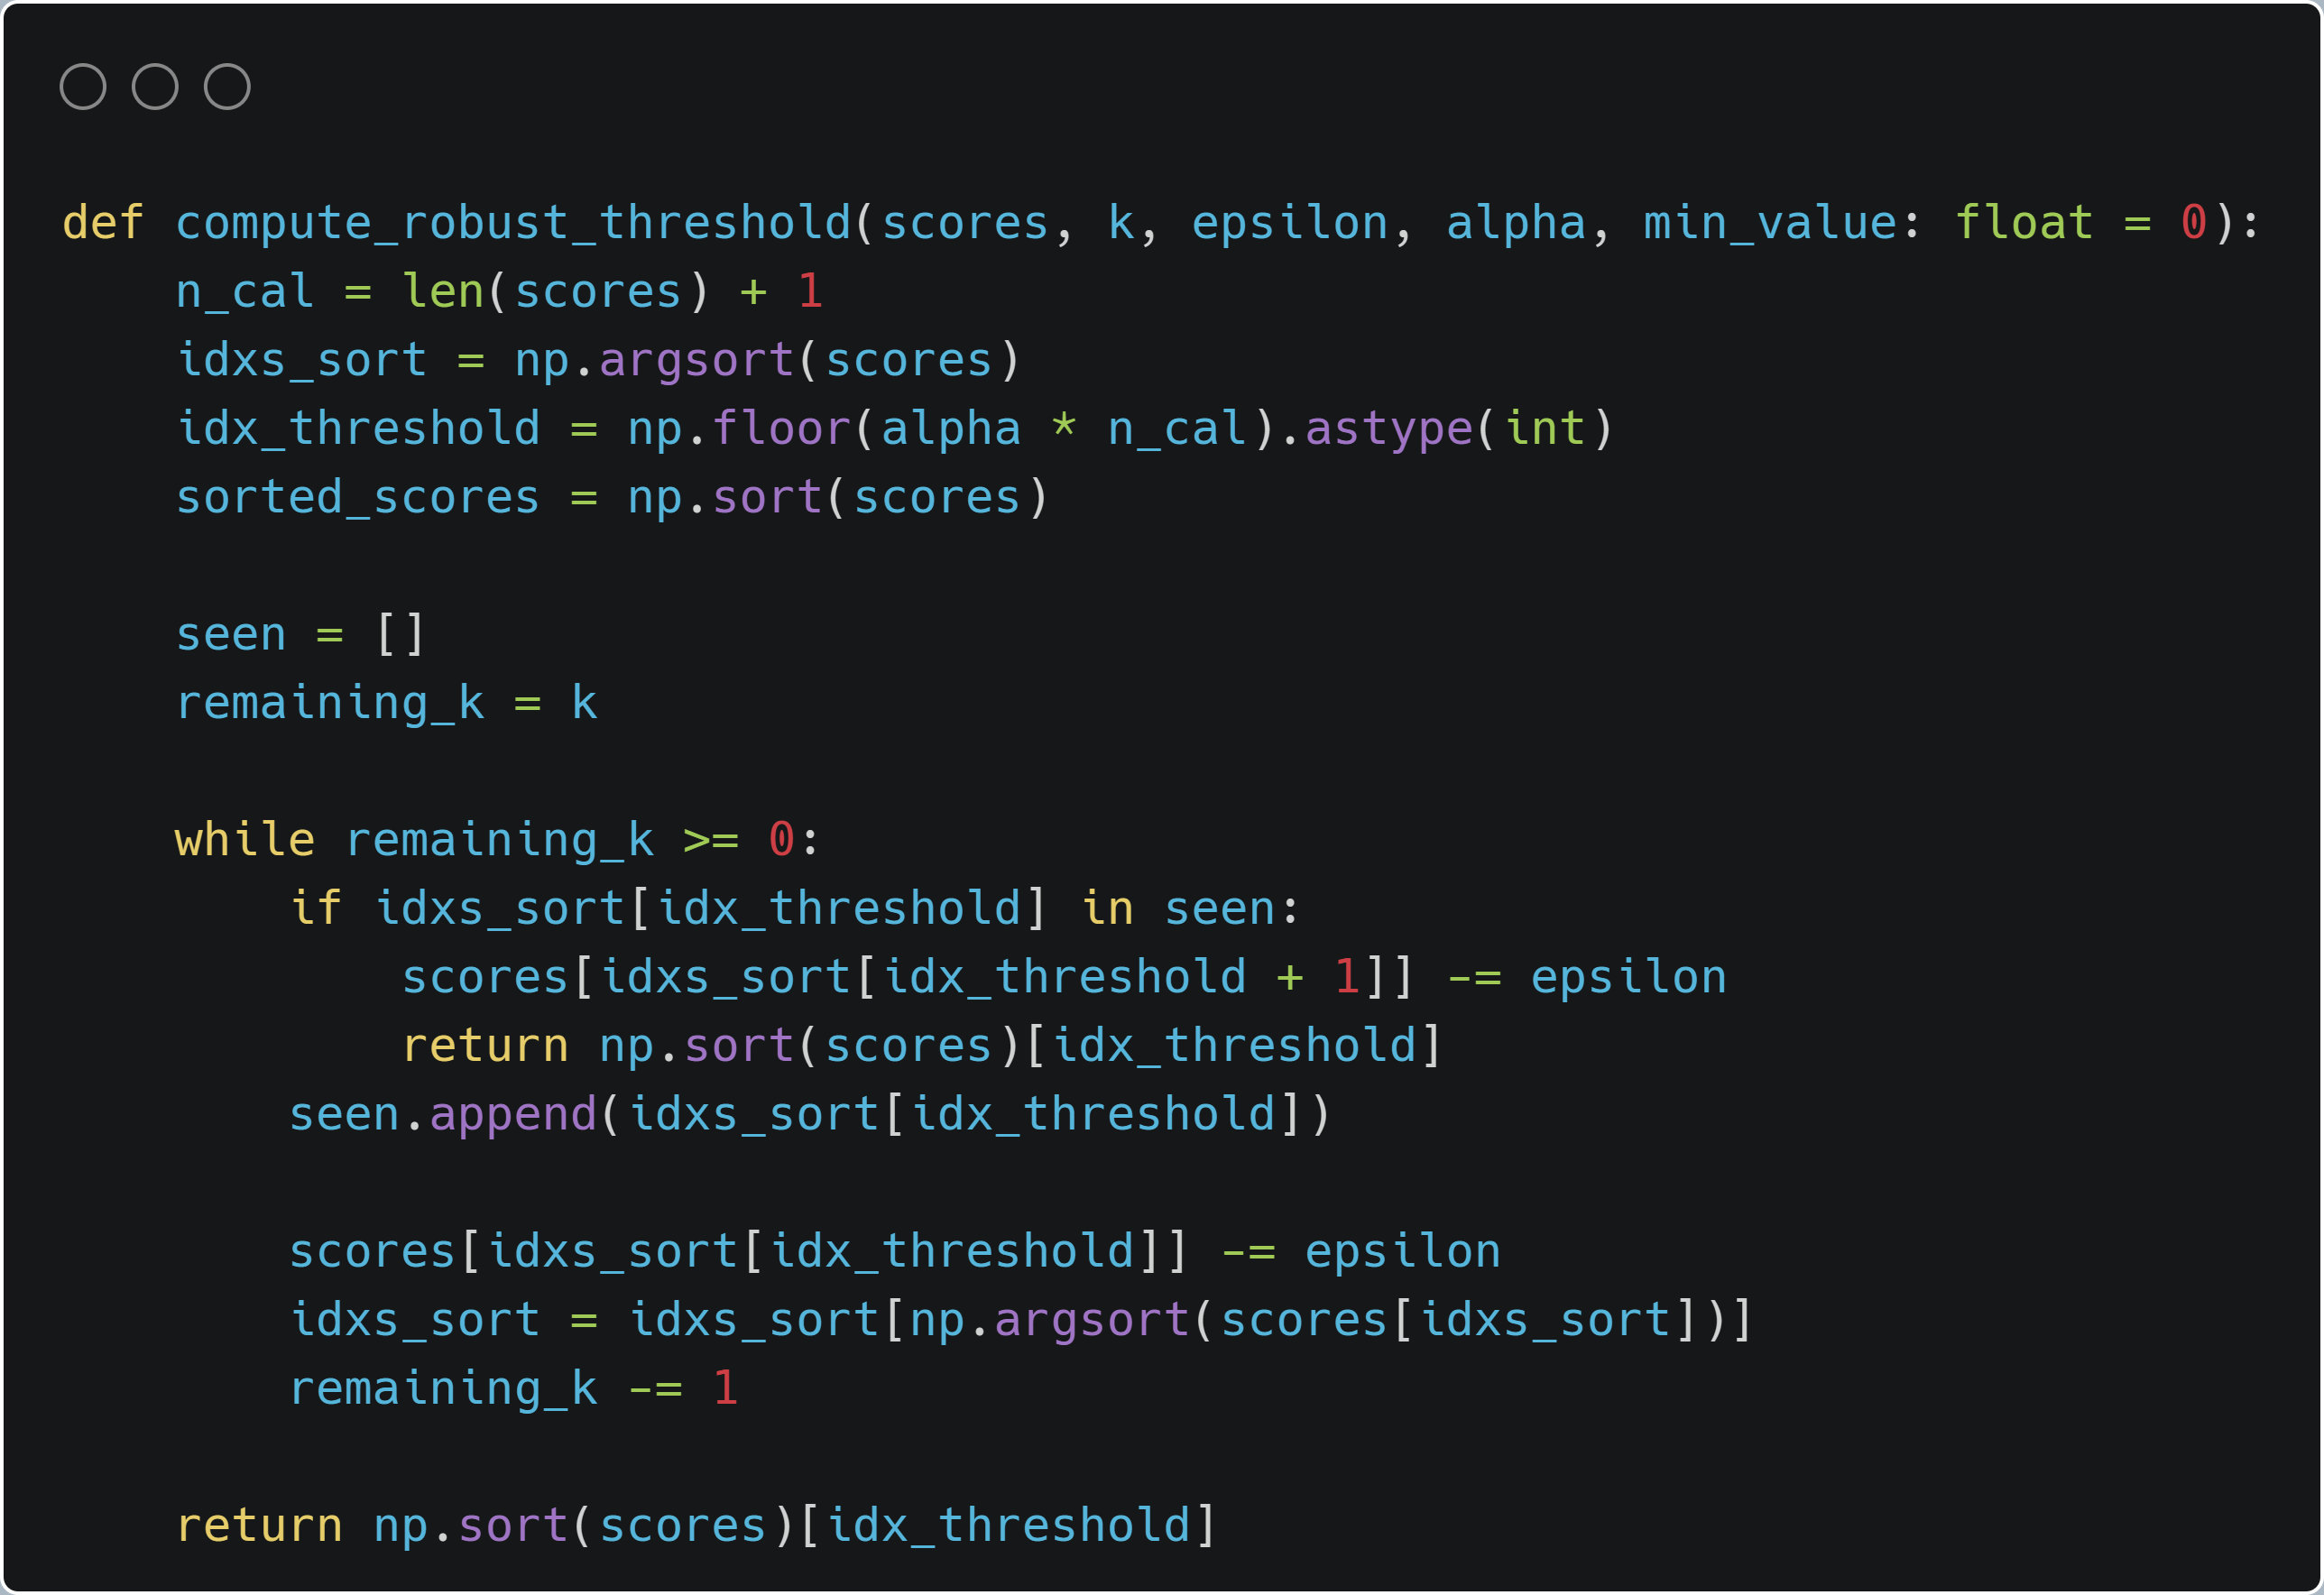
\includegraphics[width=0.5\linewidth]{poisoning_carbon.png}
    \caption{Our function for computing the maximum quantile shift and therefore certifying the robustness of prediction sets under calibration time feature poisoning attacks.}
    \label{fig:poisoning_quick}
\end{figure}


\pagebreak

\section{About the Tightness of Score Bounds}
\label{app:tightness}
To estimate how tight our score estimations are we evaluate all our methods on the same model. We train a VGG-like 1-LipNet with 10.7M parameters from \citet{boissin2025adaptiveorthogonalconvolutionscheme} on CIFAR-10. Then, we evaluate robust CP methods (average across 10 runs).

\begin{table}[h!]
  \centering
  \sisetup{
    detect-weight = true,
    detect-family = true,
    table-number-alignment = center
  }
  \begin{tabular}{
    l
    S[table-format=2.2]
    S[table-format=1.3]
    S[table-format=4.0]
  }
    \toprule
    \textbf{Method}                & {\textbf{Coverage (\%)}} & {\textbf{Set size}} & {\textbf{Runtime (s)}} \\
    \midrule
    \emph{CAS} \(n_{\mathrm{mc}}=1024\)   & 94.60                    & 2.302               & 2615                  \\
    \emph{lip-rcp}                        & 92.83                    & 1.889               &   10                  \\
    \emph{VRCP-I/C} (CROWN)               & {OOM}                    & {OOM}               & {N/A}                 \\
    \bottomrule
  \end{tabular}
  \caption{Average robust CP coverage, set size, and runtime (per run) with \(\epsilon=0.03\) across 10 runs.}
  \label{tab:robust_cp_performance}
\end{table}

CROWN does not scale to such a deep network due to its inner complexity. Additionally, given the cost of the CAS method, we did not tune the $\sigma$ smoothing hyperparameter set it to $\sigma = 2.\epsilon$ as recommended in previous works \cite{rscp_plus}. Optimizing this hyperparameter could lead to better results as obtained in \cite{bincp}.


